\articlehead{On Polynormativity}{Forneus}{2013}

It started, as these things do, with a realization about myself.

I realized that I had feelings for someone else. Not the sort of feelings that one would call ``love'', for sure, but certainly the kind that are at least as strong as your average crush-that-warrants-more-exploring. Furthermore, I felt \textit{bad} for having feelings for someone who wasn't my boyfriend, and in that kind of emotional avalanche that only humans seem to be capable of performing, I felt \textit{bad} about feeling \textit{bad} about noticing someone else. Because hey, I know several people that have multiple romantic partners, and even more people somewhere along the axis of ``I'm `attached to' one person, but we're open.''

``But wait!'', you say. ``Why is this on [adjective][species]? What does this have to do with furries at all?'' I'm glad that you asked. It turns out that furries, as a group, are incredibly polynormative.

First, a definition, if necessary: one of the great things about English is that I can make up a word like ``polynormative'' and its meaning should be immediately obvious, but in case that isn't the case, I'm defining it here as ``more accepting and understanding of poly* cultures than the mean.''

It is also relatively important that we make a distinction between ``multiple romantic partners'' and ``multiple sexual partners'', because as we'll discover, the difference in numbers is relatively significant. For the purposes of the survey, and this article, we call the former ``mono/polyamory'' and the latter ``mono/polysexuality.''

Both of these pairs are interesting, as each contains its own spectrum. The -amory spectrum runs from total monoamory, through sets of couples who consider one person to be a ``primary'' partner, to total romantic freedom. Similarly, -sexuality runs from total exclusivity, through what one commenter called ``same-room openness'' (both partners must be present, but they welcome a third or fourth sometimes), to total sexual freedom.

So now that the definitions are out of the way, let's talk numbers.

Unfortunately, the go-to group for sexuality surveys, the Kinsey Group, has done exactly one survey on polyamory and polysexuality. It's relatively fresh, being from 2000, but has one major issue: it was commissioned from Kinsey by a polyamory lifestyle magazine, and the respondents were all pulled from that magazine's subscriber base. It seems at least somewhat likely that subscribers to a poly magazine are already interested in the subject, which makes the Kinsey survey's extremely high numbers questionable. However, there are still a few things we can glean from this data: support for polyamory and polysexuality skews young, and skews male, both of which are the prime demographics of the fandom.

Even so, we should find a different source for a decent base number to compare against. One of the standard first-pass texts for people interested in polyamory and polysexuality is a book called The Ethical Slut, first published in 1997, but recently updated in 2009. This book references several studies, a few of which I'd like to highlight:

\begin{description}
  \item[The Finnish Sex Survey] indicates that 8.9\% of respondents believed that they could support a polyamorous relationship, and 8.2\% felt that it was actually best for them at their current stage of life. This survey was only given in Finland, and thus only accounts for Finnish social norms, so take that as a caveat.
  \item [Blumstein and Schwartz] report that 15-28\% of married couples surveyed allowed for non-monogamy in certain cases. This jumps to 65\% for gay men, which is highly relevant to the standard furry demographic.
\end{description}

By comparison, the numbers in the small survey we ran here at [adjective][species] paint a much different picture:

\begin{figure}
  \begin{center}
    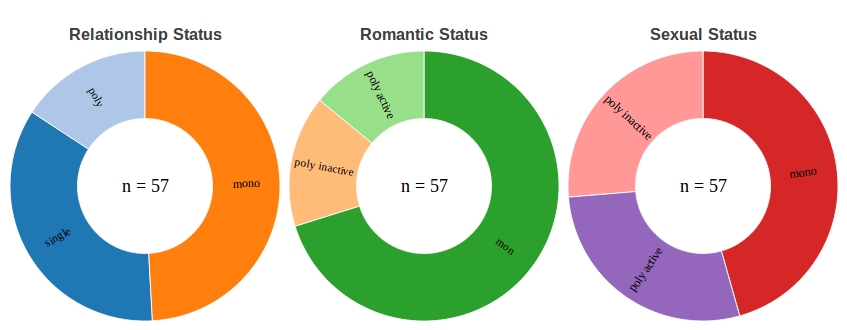
\includegraphics[width=\textwidth]{content/assets/polynormativity--results}
  \end{center}
  \caption{Monogamy/Polygamy survey results}
\end{figure}

Comparing these two gives us a few interesting points, in isolation:

\begin{itemize}
  \item Twice as many furries self-report as polysexual than as polyamorous.
  \item Three times as many furries report as polyamorous than in mainstream society.
  \item Twice as many furries self-report as polysexual than in mainstream society.
\end{itemize}

An interesting aside: before writing this article, I did an informal Twitter poll of ``do you identify as monoamorous or polyamorous, and why?'' The results, though I only got about two dozen responses, closely mirror the results of the [a][s] survey, which is great. The body of respondents very likely does too, in that, of n responses, n-1 of them were from furries. My follower ratio is slightly less furry-tilted than many that I know, at about 70/30 furry/non-furry, so we can informally posit that furries are also more likely to talk about these things, too.

To move on, I'd like to see what we can explore from the points we gleaned earlier.

\subsection*{Being a furry conditions us to think that polysexuality is more normal than the mean.}

Recently, I was at a friend's place for a weekly thing. The attendance list was ``eight furries'', as it usually is, plus or minus a few, but the point is, this is an event where furry social norms are in full force. Everyone greeted everyone else with a hug, there were 16 names for 8 people, all that jazz. At some point during the night, one of the attendants groped me. It wasn't incredibly invasive, as these things go: I told him to stop, people looked uncomfortable for three or four seconds, and that was that. He apologized, it didn't happen again, and all was good.

The interesting part of that event wasn't the event itself, but the discussions of the occurrence that happened after.

The host: ``This is why I wish that I had some more non-furry friends.''

This is a sentiment that I hear with alarming frequency, and could probably get its own entire [a][s] article. In general, it's assumed that furries are hypersexual, or at least more sexual than the average bear. This is also true of our assumptions of how the outside world sees us (ref), and statements like the one above do absolutely nothing to dispel that. ``Well, if it had been a group of you and seven other random non-furry people, they wouldn't have assumed that you were okay being touched.'' The idea being put forth here is that, as a group of furries, physical contact is expected, and therefore, we've normalized it to the point that a random grope is as mundane as a handshake is to someone outside fandom.

This is an unfortunate supposition. After all, a person who expects his personal bubble to be maintained would be offended regardless of whether or not the person doing the bubble-bursting happens to be a furry or not. Attempting to legitimize it as ``a furry thing'' does active harm to the outside perception of the fandom as oversexualized. It also does no real good for the furs inside who would prefer a more typical set of rules of engagement.

Submitted as Exhibit B: A friend who wasn't there said to me after the fact: ``Yeah, people do that to me all the time, because they assume that it's okay if I'm in a furry space.''

\subsection*{Being a non-furry operating in a mostly-furry space can skew one's perception of norms}

It's easy to see how this would be the case, but let's explore this a bit further. First, the social component: non-furries and furries alike accept the ``multiple name'' social construct to varying degrees. Personally, I attempt to find out a person's real name relatively early to avoid conversational awkwardness, as I would prefer to never have another conversation with my mother in which I have to explain why I don't know the name of the person who's crashed on our couch for three days. For a non-furry, this is even worse, as ``We spent the day with my boyfriend and his friend, uh\ldots Sheppenwolf\ldots '' is a risible statement in a great many contexts.

If we advance the clock a bit, it's easy enough to see how one can become immersed in this culture and normalize it. I, and by extension much of my social circle, have two friends that have legally changed their birth name to their furry name. Both have furry names that aren't readily identifiable as such, so it works, but in the event that they were named ``Tikkamasalacat'' or somesuch, a lot of people would shift readily. After all, we're used to using fan names as a primary mark. Mainstream society, not so much.

This translates very easily into the sexual side of the fandom, which I will discuss\ldots now.

\subsection*{Being a monogamous furry can lead to conflict with the fandom's polynormativity.}

This is something of a logical extension of the previous two, but it's worth touching on separately. At least one close friend of mine is strictly monogamous, and has expressed some discomfort at some of the standard furry social norms outlined above. This is a slightly extreme example, of course, but many people assume that it's okay to hug everyone they see at any sort of gathering, without actually asking. This probably shouldn't be the case, but many furries say that this is one of the things that they like about the fandom. Even so, one person's idea of openness is another person's idea of a popped personal bubble.

This bubble-maintenance can actually lead to some very interesting emotional backlash. Perhaps a monogamous furry feels as though he's cramping the style of the stereotypical furry by shying away from physical contact, or that maintaining monogamy is somehow counter to what the fandom wants or expects. I certainly went through a bit of this myself: early in my exploration of polyamory, I felt very weird for wanting to expand past my relationship, and that quickly evolved into ``but most of the people I know have multiple partners, so maybe I'm just doing this wrong.'' For what it's worth, while most of the people I know do in fact have multiple partners, or have at least experimented with such, this is just selection bias, even within the fandom.

There's an interesting thing to explore hiding in there, too: how 25\% became widely perceived to be a majority. Clearly, it isn't, but much like ``every man in the fandom is gay'', the assumption is often made that if you aren't naturally promiscuous, this fandom is not the place for you. There are a few possible explanations for this, at least some of which are erroneous assumptions in their own right: compare, for example, the perception that all of the art on FurAffinity is porn. It's actually somewhere around 23\% (ref), and that's ``mature'' and ``adult'' art \textit{combined}, but the fact that this is the art that gets the lion's share of the views and favorites means that the perception remains that furries are a lascivious bunch. Even if ``only'' 25\% of the furries are in open relationships, they're sometimes more vocal and certainly more visible, and that makes one more likely to think in terms of absolutes.

To conclude: the fandom's polynormative nature makes sense as an extension of its openness in other ways. We have a drastically higher percentage of people who see a hug, rather than a handshake, as the standard greeting. I would also argue that the significantly higher favorite count on adult art means that people are often not viewing it in shame. So it's pretty easy to extrapolate that to the conclusion that people who are open in general, as well as open about what they like, will be more likely to go seek that out.

The last thing to remember is that, while we are statistically more open than others, that doesn't mean that consent isn't still of paramount importance. Play safe, and communicate, just like you would expect to do within your relationship, and everyone can get along just fine.
